\chapter{Decidability Problems for Hinged Polygons and Disks}
\section{The Logic Engine}

%#History of the logic engine.  Who invented it [comsadkis???]?
\subsection{Construction of the Logic Engine and Encoding of an NAE3SAT Problem on a Logic 
Engine}
\begin{figure}[!h]
\begin{center}
%%%First Figure with armatures
\includegraphics{graphics/LogicEngineFrameFigure1Scaled.pdf}
\caption{A logic engine frame with veritical armatures and a horizontal 
shaft.}\label{fig:LogicEngineFrameFigure1.pdf}
\end{center}
\end{figure}
%#idea: SEPARATE THE CONSTRUCTION FROM THE REPRESENTATION.  AFTERWARDS TIE THE CONSTRUCTION TO 
%#REPRESENTATION
%#rigid frame - define as units of height in terms of n,m, and flag sizes (clauses, variables, and 
%#the size of qeqquilateral triangle.  the rigid frame does not move  {(x,y) | rigid frame 
%#dimensions}

% The logic engine \textit{rigid frame} is the boundar of the logic engine.  The rigid frame's center 
% is embedded at the origin of the plane and has a height of $h$ and a width of $w$.  The 
% \textit{shaft} is placed at mid-height of the rigid frame and extends the width of the frame.  The 
% \textit{armatures} are of height $h$ and are placed adjacent to each other.  
% 
% Suppose we are given an instance of an NAE3SAT, $\phi$, with $n$ 
% variables and $m$ clauses.  The logic engine is a planar model which can encode instances of the 
% NAE3SAT problem.  The components of the logic engine consists of the outermost rigid frame, the 
% shaft, the armatures, the chains, and the flags.  Figure \ref{fig:LogicEngineFrameFigure1.pdf} 
% shows the a rigid frame, armatures, and shaft.  Each armature represents a boolean variable.  The 
% rigid frame defines the border 
% of the model and the armatures has two orientations with respect to the shaft.   
\begin{figure}[!h]
\begin{center}
\includegraphics{graphics/LogicEngineFrameFigure1halfScaled.pdf}
\caption{}\label{fig:LogicEngineFrameFigure2.pdf-1}
\end{center}
\end{figure}
In figure \ref{fig:LogicEngineFrameFigure2.pdf-1}, the logic engine is flagged.  A \textit{flag} is 
 in the shape of an equilateral triangle.
%# shaft {x | 0 <=x <= xMax}





The logic engine is a planar model which can encode instances of the NAE3SAT problem.  The 
components of the logic engine are as follows: the rigid frame, the shaft, the armatures,
 and the flags.  
%Figure \ref{fig:LogicEngineFrameFigure1.pdf} shows the a rigid frame, armatures, and shaft.  
The \textit{rigid frame} is the rectangular boundary the logic engine fixed to the plane.  The 
\textit{shaft} is a horizontal line segment that is placed at mid-height of the rigid frame.  The 
\textit{armatures} are veritical line segments whose midpoints are one the shaft.  Each armature 
has two orientations with respect to the shaft.  The \textit{flags} are equilateral triangles 
attached to the armatures.  The placement of the flags is dependent on the instance of the NAE3SAT 
boolean formula. Each flag as two orientations.

For a given a boolean formula, $\Phi$, in $3-CNF$ with $n$ variables and $m$ clauses, the 
corresponding logic engine is constructed as follows: all components will be specified with a 
quantity and a size defined as polynomials in $m$ and $n$.

\begin{tabular}{|c|c|c|c|}
\hline
Component & Quantity & Size & Set Definition\\\hline
Rigid Frame&1&-&$\set{(x,y)\in\bbr^2}{\begin{array}{c}
					x \in [-\frac{1}{2}(n + 
1),-\frac{1}{2}(n+\frac{1}{2})] \cup 
[\frac{1}{2}(n+\frac{1}{2}),\frac{1}{2}(n+1)] \\
\text{ and }\\
y \in [-m - 1,-m-\frac{1}{2}] \cup 
[m+\frac{1}{2},m+1]
                                      \end{array}
                                    }$\\\hline
Shaft&1&$n+1$&$\set{(x,y) \in \bbr^2}{
\begin{array}{c}
x \in 
[-\frac{1}{2}(n+\frac{1}{2}),\frac{1}{2}(n+\frac{1}{2})]\\ 
\text{ and }\\
y=0
\end{array}
}$\\\hline
Armatures&n&-&$\set{(x,y)\in\bbr^2}{
\begin{array}{c}
x \in \left\lbrace \frac{-(n-1)}{2},\frac{-(n-1)}{2} + 1 ,\dots, 
\frac{1}{2}, \dots,\frac{(n-1)}{2} \right\rbrace\\ 
\text{ and } \\
y \in [-m,m]
\end{array}
 }$\\\hline
%Flags&-&&\\\hline
\end{tabular}
Each armature corresponds to a variable in $\Phi$. There are two literals for each variable, i.e. 
the negated literal $\bar{x}_j$ and non-negated literal $x_j$.   Flagging arragement 
indicates the relationship of the boolean literal's existence within a clause. 
\begin{enumerate}
 \item If the literal $x_j$ is found in clause $C_k$, then $l_{j,k}$ is unflagged.
 \item If the literal $\bar{x}_j$ is found in clause $C_k$, then $\bar{l}_{j,k}$ is unflagged.
\end{enumerate}

\begin{figure}[!h]
\begin{center}
\includegraphics{graphics/LogicEngineFrameFigure2Scaled.pdf}
\caption{}\label{fig:LogicEngineFrameFigure2.pdf}
\end{center}
\end{figure}

Negated literals reside below the shaft and non-negated literals reside above the shaft.
% If the NAE3SAT problem contains $m$ clauses, each armature is partitioned into $2m$ pieces.  Since the armatures represent the boolean variables, the corresponding l  $m$ pieces above the shaft and $m$ pieces below the shaft.  Each row at height $h$ above and below the shaft represents the $h^\text{th}$ clause in the boolean formula.  The flags indicate that the literal of the boolean variable does not occur in the clause, i.e.

A \textit{collision} of flags occur if either of the following occurs:
\begin{enumerate}
\item flags in the same row on adjacent armatures point toward each other.
\item a flag from the outermost armature $A_n$ points towards the outer rigid frame.
\item a flag from the innermost armature $A_1$ points inwards of $A_1$.
\end{enumerate}
\begin{figure}[!htbp]
\begin{center}
\includegraphics{graphics/logicEngineCollisions.pdf}
\caption{(a) Illustrates a adjacent flag collision at the same height, (b) and (c) illustrates a 
rigid frame collision.}\label{fig:logicEngineCollisions.pdf}
\end{center}
The logic engine representation corresponding to $\Phi$ is to be configured such that no 
horizontally adjacent flags collide and flags do not collide with the rigid frame. 
\end{figure}
\begin{figure}[!htbp]
\begin{center}
\includegraphics{graphics/logicEngineValidConfigurations.pdf}
\caption{The following configuration of adjacent flags 
and flags that are adjacent to the rigid frame.}\label{fig:logicEngineValidConfigurations.pdf}
\end{center}
\end{figure}
%define what it means to be collision-free
%explain why at least one armature is unflagged in every row.
%A row is said to be \textit{collistion-free} when 
\begin{lem}\label{lem:logicEngine1}A row has a collision-free configuration if and only if it has 
at least one unglagged armature. \end{lem}
\begin{proof}
% Do this by induction  start with 1, then suppose i flags point right, show the i+1 armature points 
% the to right.  State which types of collisions occur in the lemma.

Suppose that the the flag on armature $A_1$ is flagged.  If the flag is oriented left, then there 
is a flag-frame collision.  If the flag is oriented to the right and if $A_2$ is flagged, then 
$A_2$ must also be oriented to the right; otherwise will result in a flag-flag collision.  Now 
suppose the $i^\text{th}$ armature's flag is oriented to the right.  $A_{i+1}$ is also oriented to 
the right; otherwise will result in a flag-flag collision. By induction all flags will orient to 
the right up to $n$.  Thus the $n^\text{th}$ flag will will collide with the rigid frame.

Suppose all armatures are flagged in a row.  The flag on armature $A_1$ must point to the 
right otherwise we result in a rigid frame collision.  $A_2$ must point to the right otherwise 
we result in a rigid frame collision.  Without loss of generality, $A_i$ and $A_{i+1}$ must 
point to the right in order to prevent an adjacent flag collision.  This implies that $A_n$ 
must also point to the right which results into a rigid frame collision.

A same argument holds with the argument beginning with the flag 
on the armature $A_n$ pointing to the left.  Thus there is no collision-free configuration with 
all 
armatures flagged.


Suppose there is an unflagged armature in a row.  Turn all flags towards the nearest unflagged 
armature.  If there are flags on $A_1$ and $A_n$, point toward the interior thus they do not 
collide with the rigid frame.  If there are flags on two consecutive armatures, they do not collide 
because the nearest unflagged armature cannot be between them.  Therefore the row has a 
collision-free configuration.
\end{proof}

\begin{figure}[!h]
\begin{center}
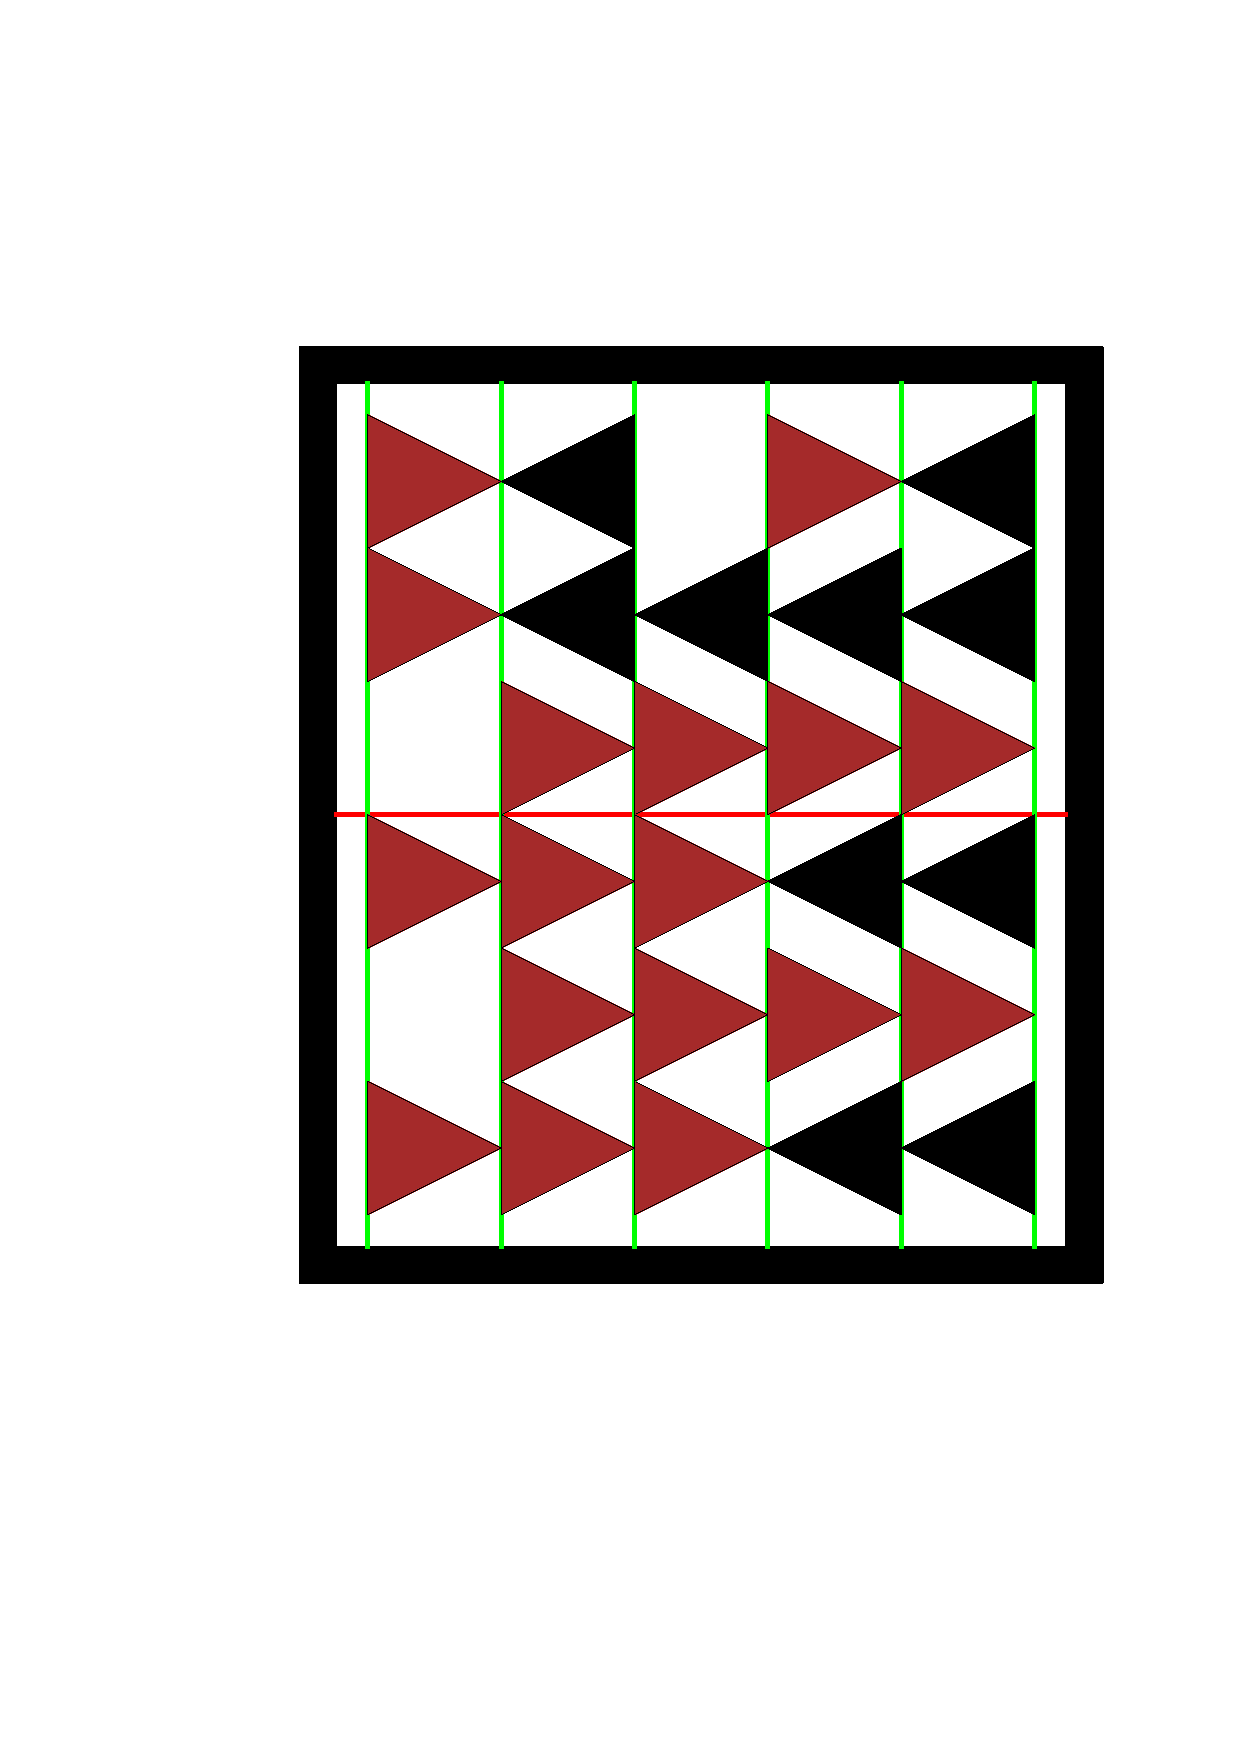
\includegraphics{graphics/LogicEngineFrameFigure5Scaled.pdf}
\caption{The logic engine from figure \ref{fig:LogicEngineFrameFigure2.pdf} whose armatures are rotated}\label{fig:LogicEngineFrameFigure5.pdf}
\end{center}
\end{figure}

%Add some introductory sentence of what happens next.  

\begin{thm}\label{thm:Satisfiability-1}
 Given an instance of a $NAE3SAT$,  it is a ``yes'' instance if and only if the corresponding logic 
engine has a collision-free configuration.
\end{thm}
\begin{proof}
Suppose we have an instance of a $NAE3SAT$ that is a ``yes'' instance. This implies that there is a 
truth assignment such that each clause contains a true and a false literal. Now consider the logic 
engine corresponding to this instance. We now 
show that it has a collision free configuration.

For variables that are true, configure the armatures such that the flags corresponding to the 
non-negated literals reside above the 
shaft and the flags that correspond to the negated literals reside below this shaft.  For variables 
that are false, configure the 
armatures in the opposite orientation.  Each clause corresponds to a pair of rows in 
the logic engine, one row for non-negated literals and one for negated literals.  Because the 
$NAE3SAT$ is a yes instance, every row contains at least one unflagged armature.  
By Lemma \ref{lem:logicEngine1}, every row  has a collision-free configuration.

Suppose we have an instance of a $NAE3SAT$ such that the corresponding logic engine has a 
collision-free configuration. By Lemma \ref{lem:logicEngine1} every row at least one unflagged 
armature.  The $k^{th}$ clause is represented by the $k^{th}$ rows above and below the shaft. If the 
literal $x_j$ is found in clause $C_k$, then the armature is unflagged in that row. If the literal 
$\bar{x}_j$ is found in clause $C_k$, then $\bar{l}_{j,k}$ is unflagged.  All flags 
corresponding to negated literals reside below the shaft and flags corresponding to non-negated 
literals reside above the shaft.  All together we have that every clause has a true literal and a 
false literal.  Thus, we have a 'yes' instance of the $NAE3SAT$.
\end{proof}
